\documentclass[tikz,border=2pt]{standalone}
\usepackage{times}
\usepackage{amsmath,amssymb}
\begin{document}
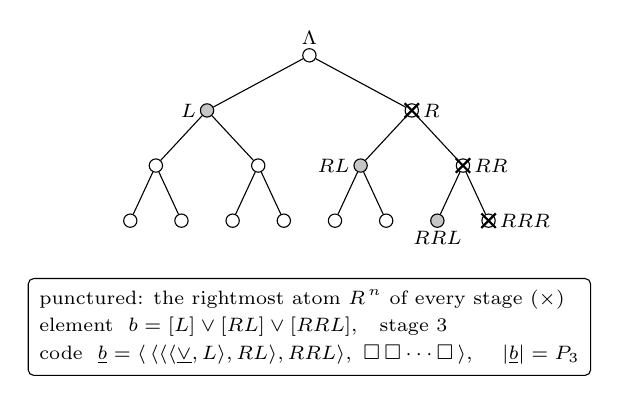
\begin{tikzpicture}[
  font=\scriptsize, level distance=7mm,
  level 1/.style={sibling distance=26mm},
  level 2/.style={sibling distance=13mm},
  level 3/.style={sibling distance=6.5mm},
  every node/.style={inner sep=1.2pt},
  sel/.style={circle, draw, fill=gray!45, inner sep=1.7pt},
  unsel/.style={circle, draw, inner sep=1.7pt}
]
\node[unsel, label=above:{$\Lambda$}] {}
  child { node[sel, label=left:{$L$}] {}
    child { node[unsel] {} child { node[unsel]{} } child { node[unsel]{} } }
    child { node[unsel] {} child { node[unsel]{} } child { node[unsel]{} } } }
  child { node[unsel] (R1) [label=right:{$R$}] {}
    child { node[sel, label=left:{$RL$}] {}
      child { node[unsel]{} } child { node[unsel]{} } }
    child { node[unsel] (R2) [label=right:{$RR$}] {}
      child { node[sel, label=below:{$RRL$}]{} } child { node[unsel] (R3) [label=right:{$RRR$}]{} } } };
% puncture the rightmost branch: cross out R, RR, RRR
\foreach \p in {R1,R2,R3} {
  \draw[thick] (\p.center) ++(-2.6pt,-2.6pt) -- ++(5.2pt,5.2pt);
  \draw[thick] (\p.center) ++(-2.6pt,2.6pt) -- ++(5.2pt,-5.2pt);
}
\node[draw, rounded corners=2pt, align=left, inner sep=4pt, font=\scriptsize] at (0,-3.45) {
  punctured: the rightmost atom $R^{\,n}$ of every stage ($\times$)\\[2pt]
  element \ $b=[L]\vee[RL]\vee[RRL]$,\quad stage $3$\\[2pt]
  code \ $\underline b=\langle\,\langle\langle\langle\underline{\vee},L\rangle,RL\rangle,RRL\rangle,\ \square\,\square\cdots\square\,\rangle$, \quad $|\underline b| = P_3$
};
\end{tikzpicture}
\end{document}
